After constructing the following model, we decided to make some additional changes in the model as follow:
\begin{itemize}
    \item Initial parameters: area = 1600 sq. ft, $E_\text{daily} = 30kWh, L_a = 1$
\end{itemize}
\begin{figure}[H]
\centering
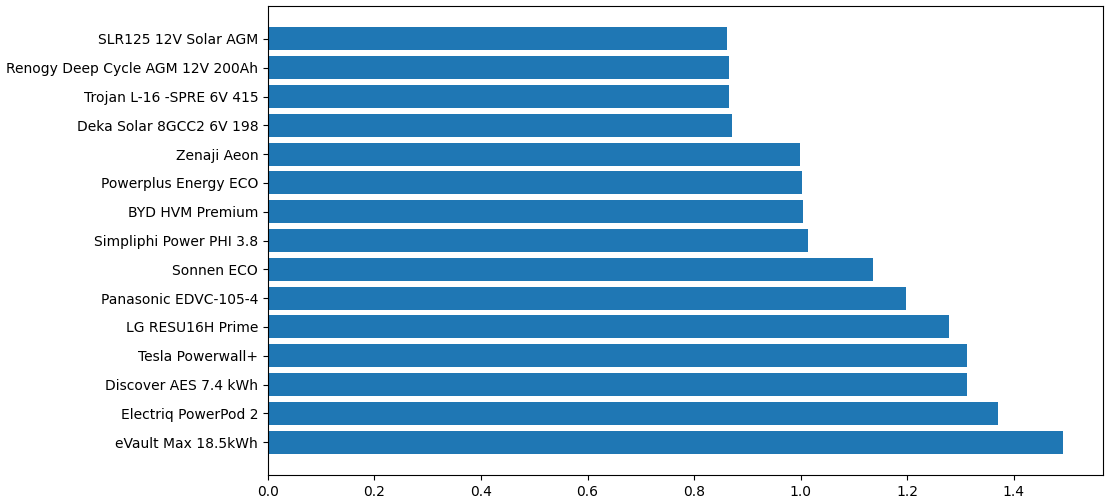
\includegraphics[scale=0.4]{src/1.png}
\end{figure}
By consulting the bar chart, one can see that there are several qualified batteries (i.e., Sonnen ECO). In addition, we also recognise batteries that have very high ratings but cannot be fully utilised (i.e., eVault Max 18.5kWh). However, it is not always the case when choosing a battery for our 1600 square-foot house. Therefore, we need to recalculate individual ratings when each factor changes. Here are several calculations on the general rating of several batteries when:
\begin{itemize}
    \item Reducing $E_\text{daily}$ to $25kWh$:
\end{itemize}
\begin{figure}[H]
\centering
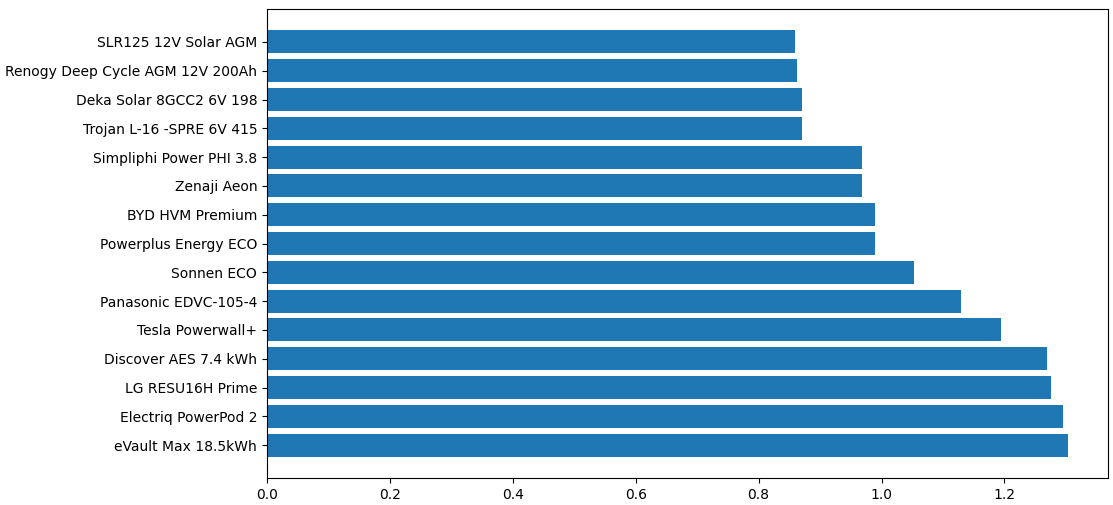
\includegraphics[scale=0.4]{src/2.png}
\end{figure}
$25kWh$ is the daily energy consumption in temperate climate areas when the weather is pleasant, and there is no demand for more electricity consumption. Therefore, the problem of choosing which battery to use will also change.
\begin{itemize}
    \item Increasing $E_\text{daily}$ to $45kWh$:
\end{itemize}
\begin{figure}[h]
\centering
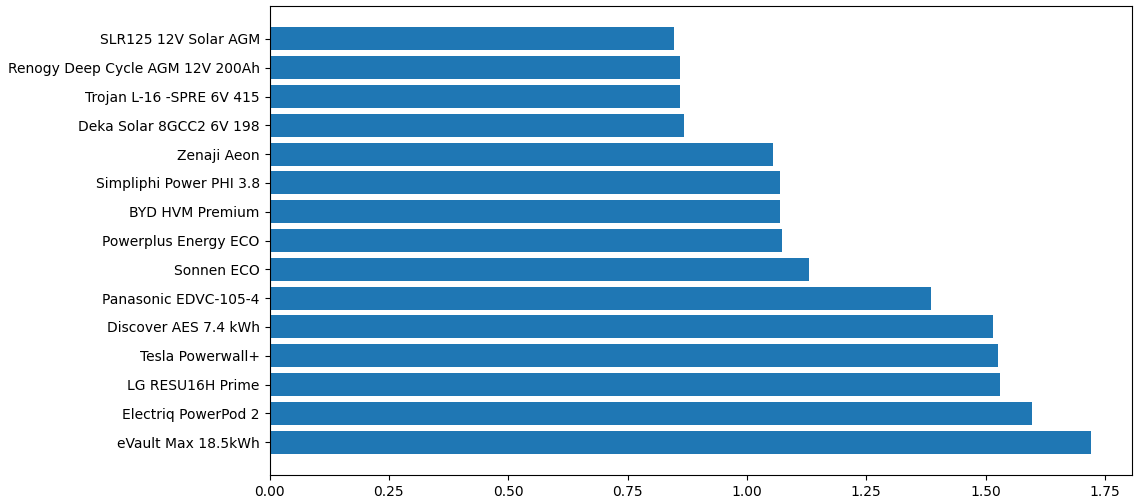
\includegraphics[scale=0.4]{src/3.png}
\end{figure}
In contrast, in several locations with extreme climates or households with many energy-intensive appliances, an increase in electrical usage is inevitable.
\begin{itemize}
    \item $L_a = 0.5 \text{days}$
\end{itemize}
In many situations, the location gets a lot of sunlight hours; therefore, the only occasion to discharge the battery is in the evening. In that case, the $L_a$ only last for 0.5 days:
\begin{figure}[H]
\centering
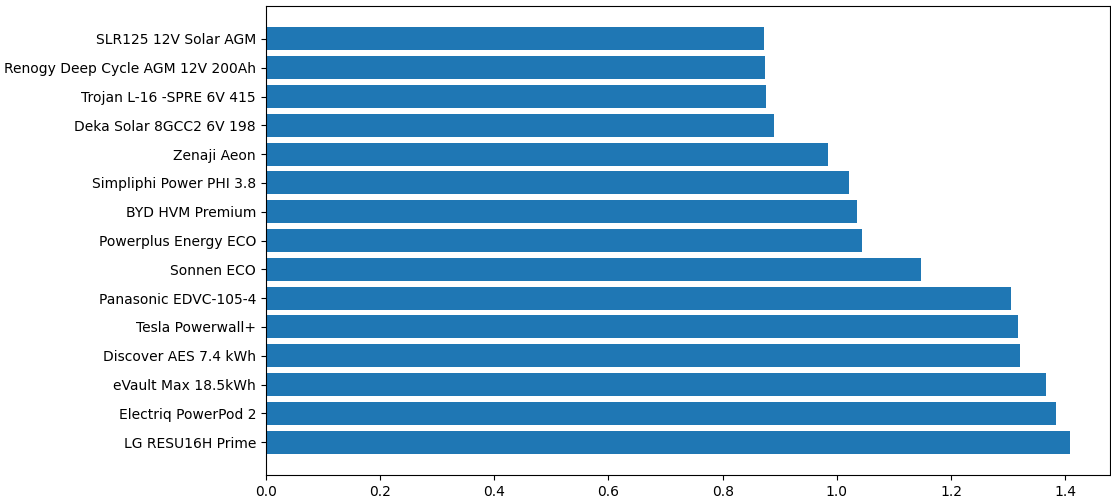
\includegraphics[scale=0.4]{src/4.png}
\end{figure}
\begin{itemize}
    \item $L_a \in \{2, 3\}$
\end{itemize}
There is a chance that there will be continuous periods of rain, so the solar system cannot capture enough energy, and you have to use the stored battery energy:
\begin{itemize}
    \item $L_a = 2:$
\end{itemize}
\begin{figure}[H]
\centering
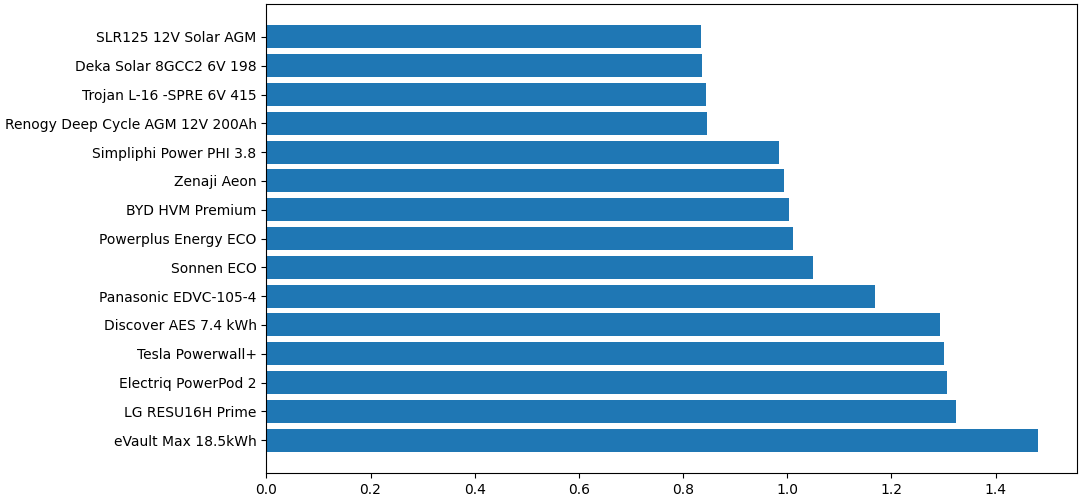
\includegraphics[scale=0.4]{src/5.png}
\end{figure}
\begin{itemize}
    \item $L_a = 3:$
\end{itemize}
\begin{figure}[H]
\centering
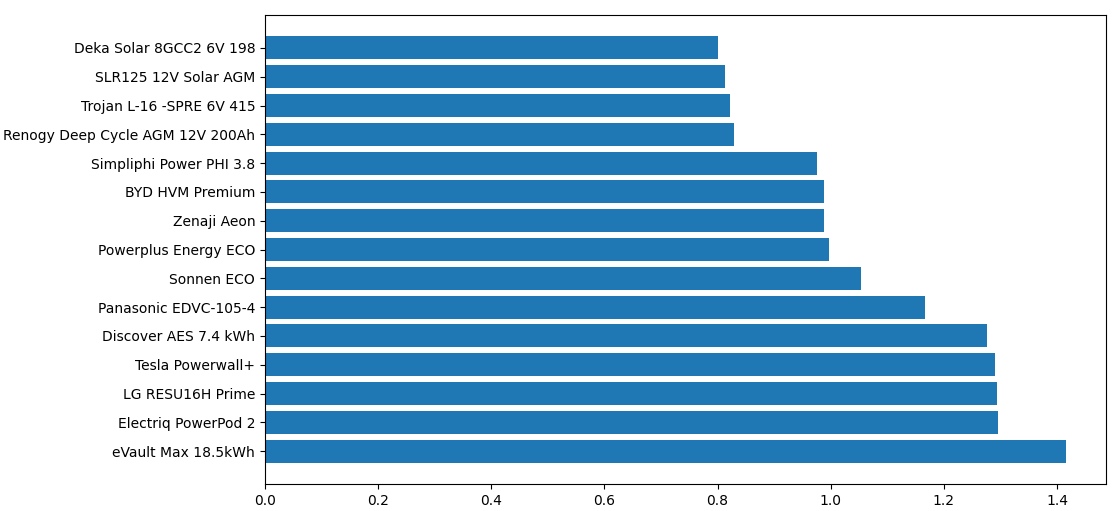
\includegraphics[scale=0.4]{src/6.png}
\end{figure}
Similar to the assumption above, we changed the state of health of all batteries to another similar value to compare more easily. However, some batteries have their lifetime inverse to their state of health's efficiency. Therefore, the assumption of the state of health will require several alterations.
\begin{itemize}
    \item $SoH = 80\%$
\end{itemize}
\begin{figure}[H]
\centering
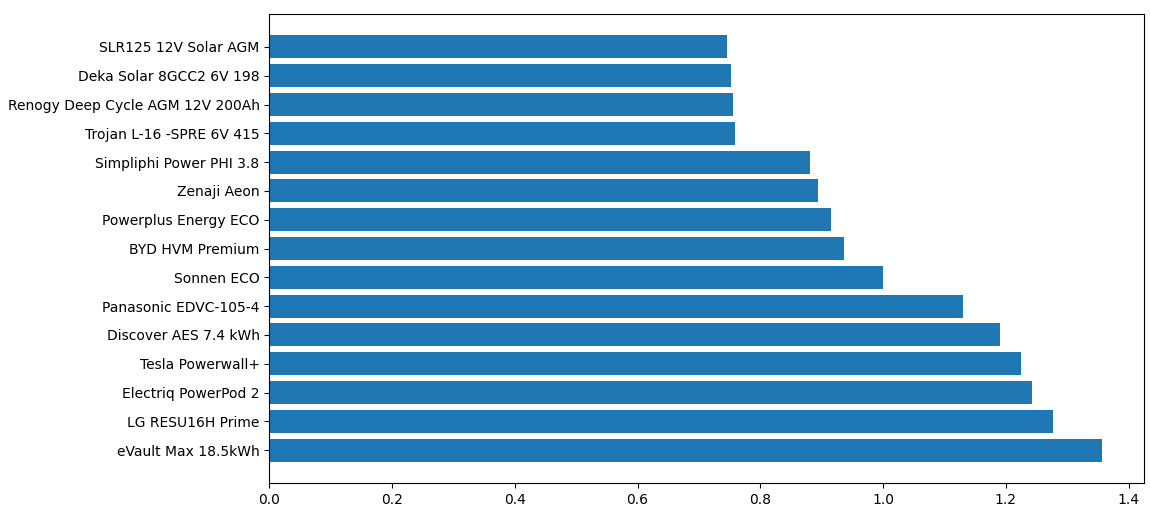
\includegraphics[scale=0.4]{src/7.png}
\end{figure}